\subsubsection{Task \& Actions}
We extend POGEMA~\cite{skrynnik2024pogema} to a budgeted hybrid-action maze navigation task with a single start-goal pair and horizon $T=100$.
At each timestep $t$, the policy outputs a continuous heading vector $a_c=(x_t, y_t)\in[-1, 1]^2$, which is discretized into the nearest cardinal direction.
The environment executes one grid move accordingly.
A discrete option $a_d \in \{\textsc{NoOp}, \textsc{Penetration}, \textsc{Boost}\}$ is available with two uses per episode, and each activation lasts two steps.
\textsc{Boost} performs two sequential sub-moves along the chosen heading, and we check for collisions after each sub-move.
\textsc{Penetration} allows the agent to traverse at most one wall cell per sub-move.
If \textsc{Penetration} expires inside a wall, the agent is relocated to the nearest free cell.

\subsubsection{States \& Rewards}
We adopt the Learn-to-Follow~\cite{skrynnik2024learn} settings to reduce exploration complexity. 
In this setup, the policy receives a waypoint sequence computed by a heuristic path decider as an auxiliary input.
The state consists of the local observation, active waypoint, and remaining option budget.
The local observation is a two-channel egocentric $m \times m$ tensor centered on the agent, where $m$ denotes the observation range.
One channel encodes walls and the waypoints, while the other encodes background agent positions.
The reward combines sparse goal-reaching terms and dense shaping with a constant timestep penalty, waypoint rewards, collision penalties, and costs for option activations.

\subsubsection{Scenarios \& Metrics}
Evaluation is conducted on three maze scenarios (Fig.~\ref{fig:environment}(a)-(c)) with increasing difficulty.

\begin{itemize}
    \item \emph{Easy}: $10 \times 10$ simple mazes with a trivial shortest path.
    \item \emph{Medium}: $20 \times 20$ mazes with complex layouts.
    \item \emph{Hard}: $20 \times 20$ non-stationary mazes with background agents that navigate with A* toward randomly sampled goals, which creates congestion and blockages around narrow passages.
\end{itemize}
Each difficulty includes ten distinct maze layouts to promote generalization.
We report \emph{Success Rate}, \emph{Time-to-Goal} (\textbf{TTG}) in decision steps with timeouts set to the episode horizon $T=100$, and \emph{Occupancy Coverage}, measured as the fraction of unique free cells visited to reflect path efficiency beyond goal completion.

\subsubsection{Training Details}
We follow the training details and network architecture of Learn-to-Follow~\cite{skrynnik2024learn}.
The agent uses a ResNet spatial encoder and MLP heads for the policy and critic, comprising approximately 5M parameters.
Action masking prevents invalid moves and option activations that violate budget or duration.
For each difficulty, the agent is trained jointly on ten maps and evaluated on unseen maps to assess generalization. 
The final policy is trained for 20 million steps, and evaluation uses the best checkpoint.

\begin{figure}[t!]
\centering
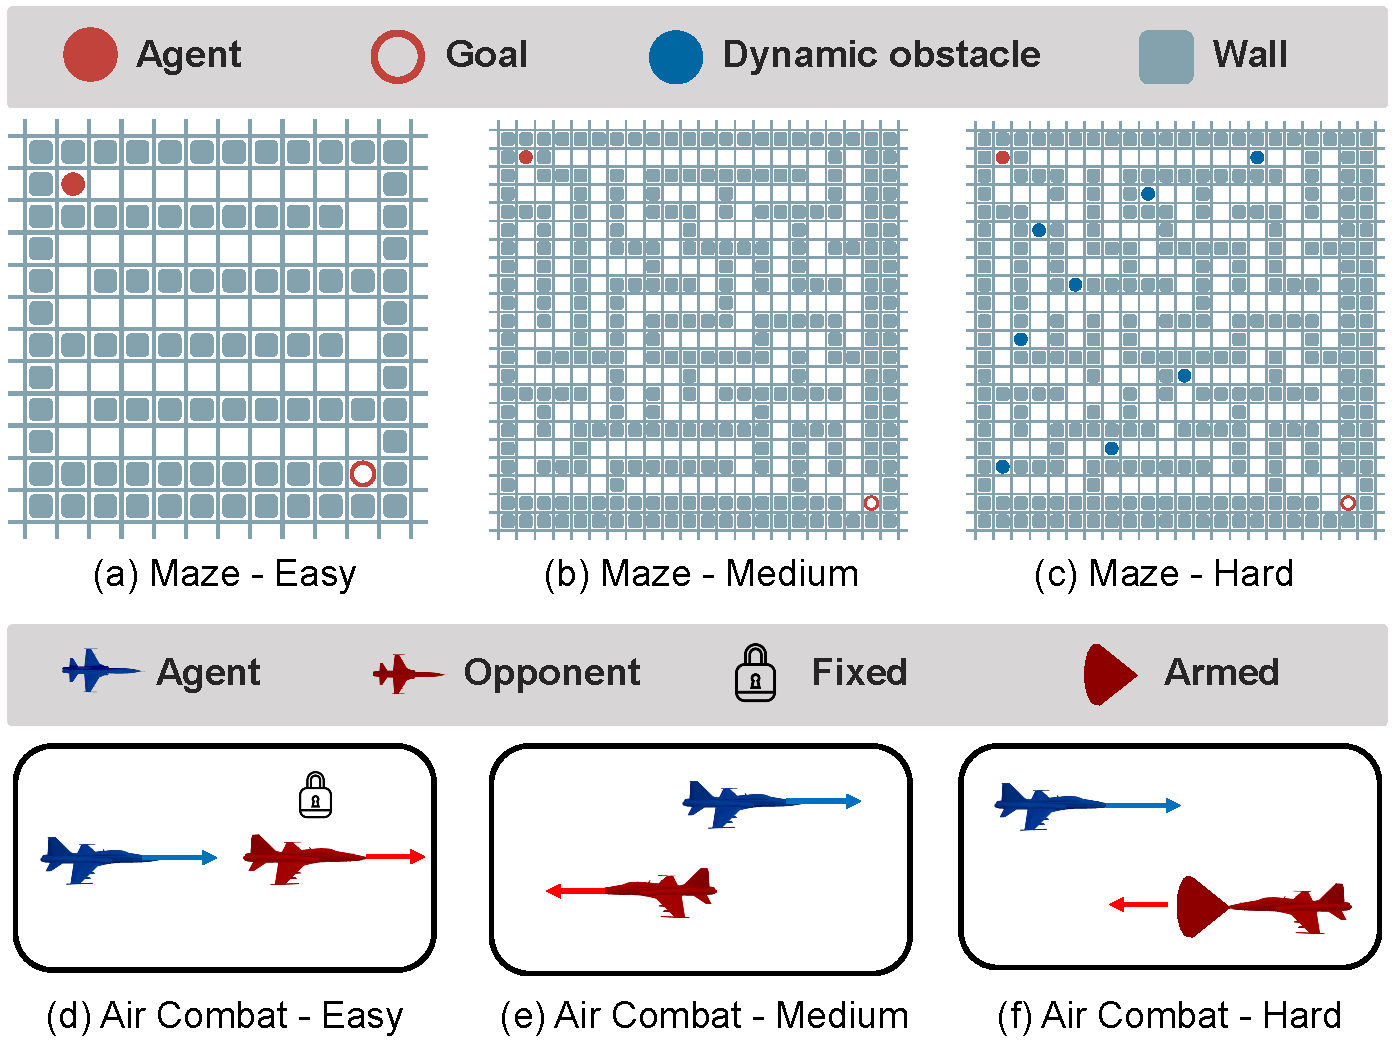
\includegraphics[width=\columnwidth]{Figures/fig_3.pdf}
\caption{Overviews and difficulty settings of the evaluation environments. 
(a)–(c) Maze Navigation: \emph{Easy} (trivially solvable), \emph{Medium} (complex), \emph{Hard} (dynamic obstacles). 
(d)–(f) Air-to-Air Combat: \emph{Easy} (fixed-maneuver opponent), \emph{Medium} (unarmed evasive opponent), \emph{Hard} (armed pursuing opponent).
}
\vspace{-10pt}
\label{fig:environment}
\end{figure}